\section{Font Size}

\subsection{Distance Dependency}

When creating graphical user interfaces one recurring question is about
what font sizes to use and what unit of measure is appropriate? Many
people still stick to pixel units, but as pixel densities vary greatly
across different devices (100 to 300ppi is quite common) it became clear
that pixel size is not a good solution. Some companies introduced device
independent pixels, but that is just the same as introducing a new
length unit like meters.

The real problem is that there is an increasing amount of different
devices around like smartphones, computer screens and digital
billboards, that are all viewed from different distances. The perceived
size of something depends on the viewing distance and this must be taken
into account.

\begin{figure}[ht]
\centering
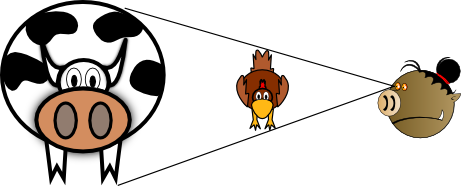
\includegraphics[width=12cm]{img/viewingdistance.png}
\caption{A chicken may be a small animal, but viewed from a nearby
distance it seems as big as a cow. }
\end{figure}

\subsection{Font Metrics}

Body height is defined as the height of the whole font, including
ascenders and descenders. In the days of metal type, the metal body of a
type had to be large enough to contain the body of a font. Due to
mechanical restrictions it also provided some extra space. So type
height is a bit larger than body height. In CSS the unit \emph{em} is
used for body height.

There is no generally accepted definition of font size. Some people
refer to it as the type height, some as the body height and others as
the cap height. As far as I know differences between type size and body
size are so small that they can be safely neglected here. When I use
\emph{font size} in this document I mean \emph{type size} as this is
common in DTP programs.

Two other important metrics are cap height and x-height. Cap height is
the height of the capital letter \emph{H} while x-height is the height
of the small letter \emph{x}. Cap height is important, because it can
easily be measured and some experts have used it to recommend ergonomic
font sizes. Other people point out that x-height is more important for
readability, but as I only know recommendations for cap height, I will
stick to cap height instead of x-height throughout this document.

\begin{figure}[ht]
\centering
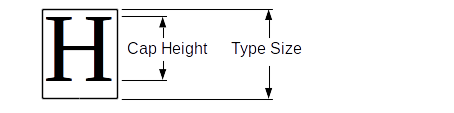
\includegraphics[width=12cm]{img/fontmetrics.png}
\caption{Type size of a font. The type size is larger than the
size of a capital letter.}
\end{figure}

The size of a font is usually measured in point (pt). There are a lot
of different point units, but nowadays the most commonly used is the DTP
point.

$$ 1 point = 0.353 mm $$

Many traditional fonts were created according to the same rules of
typesetting. Fonts adhering to the American Pica system often satisfy
the following equations:

$$ cap\ height = type\ size \cdot 0.71 $$
$$ type\ size = cap\ height \cdot 1.41 $$

From this formulas we can calculate the cap height for some type sizes
and get this nice table, which will come in handy later:

\vspace{1em}
\begin{tabular}{rrr}
Type Size (pt) & Cap Height (pt) & Cap Height (mm)\\[0.5ex]
8 & 5.7 & 2\\
9 & 6.4 & 2.25\\
10 & 7.1 & 2.5\\
11 & 7.8 & 2.75\\
12 & 8.5 & 3\\
13 & 9.2 & 3.25\\
14 & 9.9 & 3.5\\
15 & 10.7 & 3.75\\
16 & 11.4 & 4\\
17 & 12.1 & 4.25\\
18 & 12.8 & 4.5\\
19 & 13.5 & 4.75\\
20 & 14.2 & 5
\end{tabular}
\vspace{1em}

LaTeX uses a font size of 10pt as a standard for books and this size is
commonly used today. 8pt has traditionally been the smallest size used
for book printing.

Remember that the above table is not valid for all fonts. The actual cap
height depends on the individual font. Especially fonts designed for
reading on a computer screen often utilize larger cap and x-heights to
increase readability.

\subsection{Viewing Distances}

Lets take a look at some typical viewing distances for different
activities:

\vspace{1em}
\begin{tabular}{lr}
Activity & Viewing Distance\\[0.5ex]
Book reading & 30 to 40cm\\
Working at a desktop computer & 60 to 80cm\\
Looking at a billboard & many meters\\
\end{tabular}
\vspace{1em}

When people are reading a small book they often get immersed and hold it
quite near before their eyes. 30cm is the distance used by
ophthalmologists, when conducting tests with the Amsler grid. It is also
the nearest point people in the mid forties typically can focus. This is
why older people usually need glasses for reading.

60 to 80cm as a viewing distance for desktop computers may seem quite
large to many readers, but it is commonly recommended, for example by
the German VBG (Verwaltungs Berufsgenossenschaft). The reason for such
distances is to reduce strain on the eye and to enable a healthy and
relaxed working position.

One important lesson is, that font sizes for desktop computer screens
should be about twice as large as font sizes for books. The smallest
print used for books throughout the centuries has been 8pt (2mm cap
height). So the recommended minimum font size for effortless reading
from a screen is 16pt (4mm cap height). Some people may think, that this
is ridiculously large, but viewed from the recommended distance a 16pt
font on a screen appears the same size as an 8pt font in a book.

\subsection{Recommended Font Sizes}

Experts have conducted experiments to find out the optimal font sizes
for reading. The German VBG (Verwaltungs Berufsgenossenschaft)
recommends a cap height of 22 to 31 minutes of arc. For typical viewing
distances this results in the following table:

\vspace{1em}
\begin{tabular}{rrr}
Viewing Distance & Min Cap Height & Max Cap Height\\[0.5ex]
30cm & 1.93mm & 2.72mm\\
35cm & 2.26mm & 3.18mm\\
40cm & 2.58mm & 3.64mm\\
50cm & 3.23mm & 4.55mm\\
60cm & 3.87mm & 5.45mm\\
80cm & 5.16mm & 7.27mm\\
1m & 6.45mm & 9.09mm
\end{tabular}
\vspace{1em}

This does not mean that smaller sizes are unreadable, but smaller sizes
are harder to read and require more time. The same goes for fonts that
are too large.

\subsection{Cap and Rem Units}

ui2go tries to make life easier for programmers, so that they don't have
to think much about different font sizes. Therefore it introduces two
additional units of measure (sorry for that): cap and rem. Cap is the
recommended height for capital letters in a standard font and Rem is the
recommended size of em (or type height as I assume, that they are nearly
the same).

$$ 1 cap = viewing\ distance(in\ mm) \cdot 7 / 1000 $$

$$ 1 cap = 24 minutes\ of\ arc $$

$$ 1 rem = viewing\ distance(in\ mm) / 100 $$

The standard layout manager supports both units, so that they can be
used directly. But does this really work in practice? Here are some
examples to give you the idea:

\begin{enumerate}
\item
  For a viewing distance of 30cm one cap results to 2.1mm. That's
  slightly larger than the smallest size used in traditional print.

  30cm is also a typical smartphone distance and one rem at this
  distance is 3mm. This corresponds to 16dp (device independent pixel)
  on an Android device. It is the typical
  \href{http://developer.android.com/design/style/metrics-grids.html}{type
  size for text on a button}.
\item
  Imagine yourself sitting in a diplomatic conference, important papers
  lying in front of you on the table. Of course you don't want to pick
  up the papers and hide yourself or even worse, bow down (in front of
  whoever) to read them.

  What would you do? The typical viewing distance is about 50cm, the
  result for one cap is 3.5mm. This corresponds to a 14pt font. It comes
  as no surprise that US diplomatic documents actually
  \href{http://en.wikipedia.org/wiki/Times_New_Roman}{use 14 point
  fonts}.
\item
  At 60cm we get a cap height of 4.2mm, a typical value recommended for
  effortless reading on a desktop computer screen.
\item
  When looking at a billboard viewing distances are typically many
  meters. At 100 meters one rem (type size) is 1 meter. This translates
  roughly to 30 inches of cap height for a distance of 300 feet.

  This is the well known rule of thumb known to US billboard designers:
  1 inch of letter height provides best impact at a distance of 10 feet.
\end{enumerate}

Conclusion: Caps and rems really do the trick and might prove as a
valuable help for interface design in the future.

